\chapter{Shortcomings of Korat}
This chapter presents two scenarios where Korat fails to generate the best possible results it is capable of producing with its algorithm. The first example shows how Korat malfunctions by terminating before exploring all the states when reflection is used in the predicate written by the programmer. The second example shows how korat explores more states than required when the predicate written by the programmer doesn’t return the result as soon as possible. Both examples use a binary tree data structure to illustrate a predicate method that validates a linked data structure. The shortcomings observed in both the examples will also apply for an array-based data structure, like a heap.

\section{Usage of reflection for field access}
In this example, we use two different ways of field access using reflection to illustrate both the ways a programmer can use reflection to access a field. Figure 2-1 shows the java code  for a binary tree implementation. Each object of the class BinaryTree represents a binary tree. The value of the size field is the number of nodes in the tree. Objects in the inner class Node represent nodes of the tree. To use Korat, the programmer needs to provide an imperative predicate that checks the validity of inputs. It is called repOk and it typically checks the representation invariant or class invariant of the corresponding data structure. \\


\begin{figure}
\centering
\begin{lstlisting}[language=Java]
class BinaryTree {
    Node root;    // root node
    int size;    // number of nodes in the tree
    static class Node {
        Node left;    // left child
        Node right;    // right child
    }

    boolean repOK() {
        // checks that empty tree has size zero.
        if (root == null) return size == 0;
        Set visited = new HashSet();
        visited.add(root);
        LinkedList workList = new LinkedList();
        workList.add(root);
        // loop checks that the object graph is a tree.
        while (!workList.isEmpty()) {
            Node current = (Node) workList.removeFirst();
            if (current.left != null) {
                if (!visited.add(current.left)) return false;
                workList.add(current.left);
            }
            if (current.right != null) {
                if (!visited.add(current.right)) return false;
                workList.add(current.right);
            }
        }
        // checks that the size is consistent.
        return (visited.size() == size);
    }
}
\end{lstlisting}
\caption{Binary tree example with repOk using direct field access.}
\label{fig:btreeDirectRepOk}
\end{figure}

\par
Figure 2-1 also shows the repOk method that uses direct field access for BinaryTree; repOk is a predicate that checks the input is indeed a valid binary tree with the correct size. First, repOk checks if the tree is empty. If not, repOk checks that there are no undirected cycles in the object graph reachable from the root field along the left and right fields. It finally checks that the number of nodes reachable from the root is the same as the value of field size. The programmer can use Korat to generate valid test inputs for any method that requires a BinaryTree instance as an input. Each binary tree generated will satisfy the repOk. To limit the number of inputs, the programmer provides Korat with a finitization that specifies bounds on the number of objects in the data structures and on the values in the fields of these objects. For trees, the finitization specifies the maximum number of nodes and the possible elements. A tree is considered to be in scope n, if it has at most n nodes and n elements. We can use integers from 1 to n for the size field inside the BinaryTree class.

\par
Given a finitization and a value for scope, Korat generates all non-isomorphic structures that can be formed for a given data structure. In our example, two binary trees are isomorphic if they have the same underlying graph and the elements, irrespective of the identity of the actual nodes in the trees. 

\begin{figure}
\centering
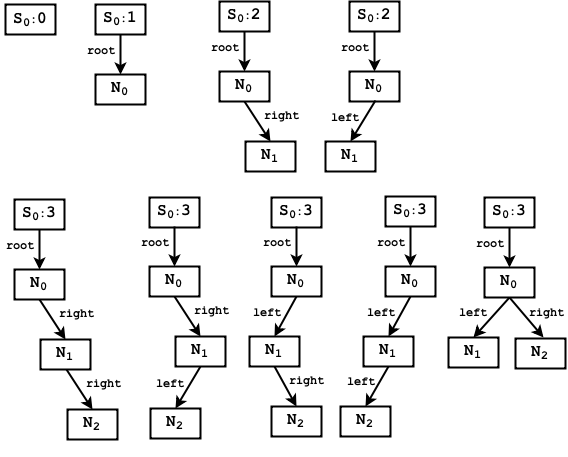
\includegraphics[width=12cm,height=8cm,keepaspectratio]{korat_instances_binary_tree_size_3}
\label{fig:btreeKoratGenScopeThree}
\caption{Binary trees that Korat generates for scope three.}
\end{figure}

\par
When using the repOk shown in Figure 2-1 with a scope of three, Korat generates 90 non-isomorphic candidate structures of which 9 structures end up being valid as they pass the repOk. Figure 2-2 shows the trees that Korat generates for scope three. Each tree consists of one BinaryTree object S0 and upto three Node objects (N0, N1, N2). For each object, the value and the identity of primitive fields and Node objects is shown. Edges represent the values of reference fields with no edge for null.

\par
To enable efficient search for valid structures, Korat encodes each structure with a state, and each finitization bounds the state space. Korat uses backtracking to systematically search this state space to find all valid structures. Based on a finitization for the input structures of the predicate, Korat first initializes the state space of structures. Korat then builds candidate structures and executes the predicate on them to check their validity. Korat monitors these executions to dynamically determine which parts of the candidate the result of the predicate depends on. More specifically, Korat monitors the fields of the candidates the execution accesses. If the predicate returns true, Korat outputs the candidate as a valid structure for testing. Otherwise, if the predicate returns false or an exception is thrown in the middle of execution, Korat skips the candidate. Korat then backtracks on the values of the accessed fields, to generate the next candidate. Finally, Korat terminates when it explores the entire search space. 

\begin{figure}
\centering
\begin{lstlisting}[language=Java]
boolean repOK() {
    // checks that empty tree has size zero.
    if (root == null) return size == 0;
    Set visited = new HashSet();
    visited.add(root);
    LinkedList workList = new LinkedList();
    workList.add(root);
    // loop checks that the object graph is a tree.
    while (!workList.isEmpty()) {
        Node current = (Node) workList.removeFirst();
        if ((Node)BinaryTree.class.getDeclaredField(``left'')
            .get(current) != null) {
            if (!visited.add(current.left)) return false;
            workList.add(current.left);
        }
        if (current.right != null) {
            if (!visited.add(current.right)) return false;
            workList.add(current.right);
        }
    }
    // checks that the size is consistent.
    return (visited.size() == size);
}
\end{lstlisting}
\caption{RepOk using the java reflection API for accessing the left child of a Node inside the loop.}
\label{fig:btTreeReflectionRepOK}
\end{figure}

\par
Korat monitors field accesses by replacing direct field accesses with accessor methods that make note of the access and hence affect the way Korat generates candidates. Figure 2-3 and figure 2-5 show repOKs that use reflection to access fields in the BinaryTree class.

\begin{figure}
\centering
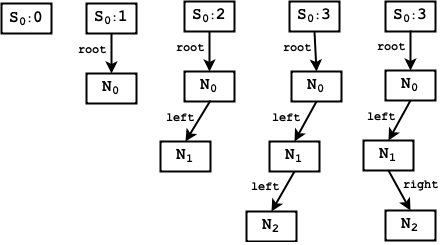
\includegraphics[width=11cm,height=6cm,keepaspectratio]{korat_instances_reflection_binary_tree_size_3}
\label{fig:btreeReflectKoratGenScopeThree}
\caption{ Binary trees that Korat generates for scope three when repOk uses reflection.}
\end{figure}

\par
The main difference between the repOk that uses direct access (shown in figure 2-1) and the repOk that uses the java reflection API (shown in figure 2-3) is the access of just one field.The latter repOk accesses the left child of every Node object using the java reflection API instead of direct field access. Since Korat is capable of monitoring only direct field accesses, it doesn’t account for this field access. This ends up affecting the generation of candidates and produces fewer trees than the direct access repOK, for the same scope. Figure 2-4 shows the binary tree structures generated when the repOk in figure 2-3 is used to validate the binary tree candidates that Korat explores. Korat generates only 28 non-isomorphic candidate structures of which 5 structures end up being valid as they pass the repOk.

\begin{figure}
\centering
\begin{lstlisting}[language=Java]
boolean repOK() {
    // checks that empty tree has size zero.
    if (root == null) return size == 0;
    Set visited = new HashSet();
    visited.add(root);
    LinkedList workList = new LinkedList();
    workList.add(root);
    // loop checks that the object graph is a tree.
    while (!workList.isEmpty()) {
        Node current = (Node) workList.removeFirst();
        if ((Node)ReflectionUtils
            .getFieldValue(current, ``left'') != null) {
            if (!visited.add(current.left)) return false;
            workList.add(current.left);
        }
        if (current.right != null) {
            if (!visited.add(current.right)) return false;
            workList.add(current.right);
        }
    }
    // checks that the size is consistent.
    return (visited.size() == size);
}
\end{lstlisting}
\caption{RepOk using the user written reflection API for accessing the left child of a Node inside the loop.}
\label{fig:btTreeUserReflectionRepOK}
\end{figure}

\par
This proves that Korat’s algorithm is drastically affected even if a single field access is done using reflection. To make sure Korat functions as expected and continues to remain complete, it is essential to account for field accesses that use reflection, including direct field accesses. Figure 2-5 shows another version of repOk that uses a user written method to access the left field of every Node object. It is assumed that this method uses java reflection API within the method body. Using this version of repOk to generate binary tree inputs also produces the same trees shown in figure 2-4 as Korat is capable of monitoring only direct field accesses. 


\section{Inefficient predicates}
Korat claims to efficiently generate all valid non-isomorphic structures even for large state spaces. The search pruning that Korat performs allows Korat to explore only a tiny part of the state space. The ratio of the number of candidate structures considered and the size of the state space shows that the key to effective pruning is backtracking based on fields accessed during predicate execution. Korat usually performs extremely well when the user written predicate returns a true/false as soon as it knows the result. Figure 2-1 shows a repOk of a BinaryTree that checks for three violations that can render a candidate as an invalid binary tree. The repOk returns false as soon as it knows that the candidate has violated one of the three rules for a graph to be a binary tree.

\begin{figure}
\centering
\begin{lstlisting}[language=Java]
boolean repOK() {
    boolean result = true;
    // checks that empty tree has size zero.
    if (root == null) result = (size == 0);
    Set visited = new HashSet();
    LinkedList workList = new LinkedList();
    if (root != null) {
        visited.add(root);
        workList.add(root);
    }
    // loop checks that the object graph is a tree.
    while (!workList.isEmpty()) {
        Node current = (Node) workList.removeFirst();
        if (current.left != null) {
            if (!visited.add(current.left)) result = false;
            else workList.add(current.left);
        }
        if (current.right != null) {
            if (!visited.add(current.right)) result = false;
            else workList.add(current.right);
        }
    }
    // checks that the size is consistent.
    if(!result) result = (visited.size() == size);
    return result;
}
\end{lstlisting}
\caption{RepOk that doesn’t return the result as soon as it knows it.}
\label{fig:bTreeInefficient}
\end{figure}

\par
When using the repOk shown in Figure 2-1 with a scope of three, Korat generates 90 non-isomorphic candidate structures of which 9 structures end up being valid. The repOk shown in figure 2-5 has the exact same functionality and also generates the same valid structures as the repOk in figure 2-1 but, it ends up generating 893 candidate structures for scope three which is an order of magnitude more than the number of candidate structures generated by the repOk in figure 2-1. For a larger scope, we can observe an increase by multiple orders of magnitude. The repOk in figure 2-5 ends up being an inefficient predicate for generation as it does not return true/false right after it knows the result. This is one of the reasons why Korat doesn’t make any promises about its efficiency as it is partly dependant on the predicate written by the user. Though this is not a shortcoming of Korat, it is one of the situations where the effectiveness of Korat is nullified.
